\chapter{Практическая часть}

\section{Создание проекта}
На рисунках ниже представлен процесс создания проекта.
\begin{figure}[H]
    \centering
    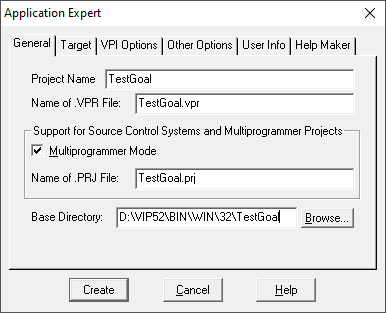
\includegraphics[scale=.7]{data/image/gen_1.png}
    \caption{Создание нового проекта.}
\end{figure}
\begin{figure}[H]
    \centering
    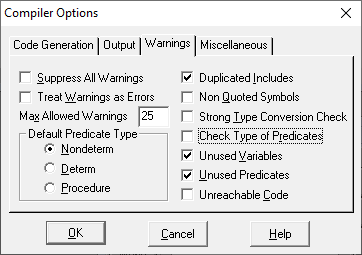
\includegraphics[scale=.7]{data/image/gen_2.png}
    \caption{Настройка проекта.}
\end{figure}
\begin{figure}[H]
    \centering
    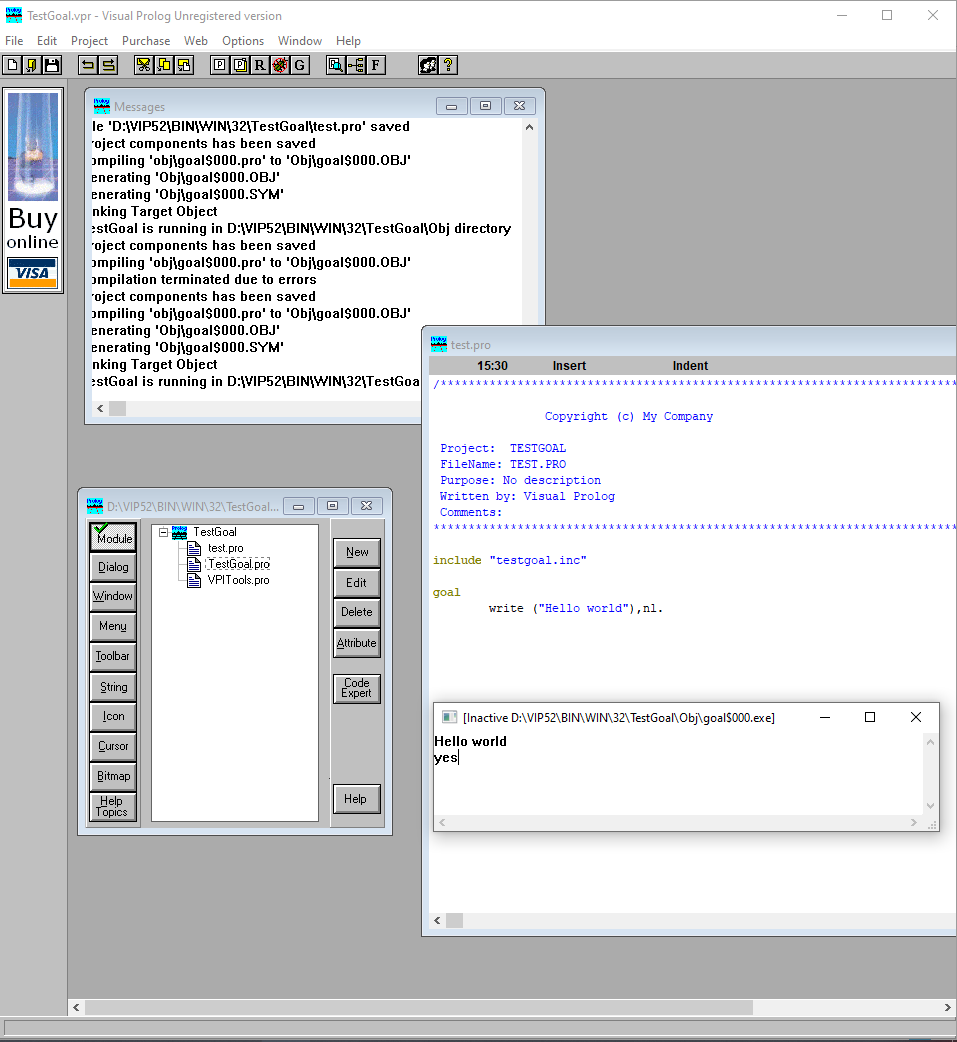
\includegraphics[scale=0.6]{data/image/gen_3.png}
    \caption{Запуск тестовой программы.}
\end{figure}

\section{Задание:}
запустить среду Visual Prolog5.2. Настроить утилиту TestGoal. Запустить тестовую программу, проанализировать реакцию системы и множество ответов. Разработать свою программу -- <<Телефонный справочник>>. Протестировать работу программы.

На листинге ниже представлен текст разработанной программы.

\lstset{language=python}
\begin{lstlisting}[caption=Текст программы]
domains
   name = symbol
   number = integer

predicates
  phonebook(name,number)

clauses
  phonebook(tolya, 111111111).
  phonebook(kolya, 222222222).
  phonebook(olya, 333333333).
  phonebook(sasha, 444444444).
  phonebook(misha, 555555555).
  phonebook(dasha, 666666666).
  phonebook(olya, 777777777).

goal
  %phonebook(dasha, Phone).
  phonebook(olya, 333333333).
\end{lstlisting}

\textbf{Примеры работы:}
\begin{enumerate}
    \item Если имя встречается в телефонном справочнике один раз.
\begin{figure}[H]
    \centering
    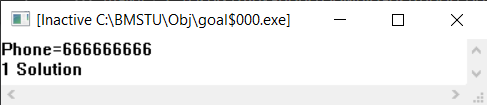
\includegraphics[scale=1.5]{data/image/1.png}
    \caption{phonebook(dasha, Phone).}
\end{figure}

    \item Проверка корректности телефонного номера.
\begin{figure}[H]
    \centering
    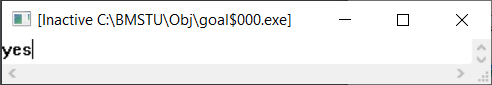
\includegraphics[scale=1.5]{data/image/2.png}
    \caption{phonebook(olya, 333333333).}
\end{figure}
\end{enumerate}
